\chapter{Parallel architectures (temporary title)}


\section{Introduction}

% [Quels sont les buts de ce chapitre: 
% - Introduire le calcul parallèle et ses applications generales, et plus precisement pour les systemes d'equation larges
% - Parler des différents types d'architecture parallèle tout en indiquant leur utilité generale, et leur adéquation avec les systemes d'equation larges
% - Parler des environnements de developpement parallèle et ceux qui sont les plus à même de gerer des systemes d'équations larges sur les systemes distribué
% ]

Parallel computing is a method that enable  running multiple processes concurrently on one or multiple process units, tackling the limitations of sequential computation, by allowing treatment of growing data volumes and computational demands. Back to the mid-20th century, the computation was solely based on sequential architecture that enables the execution of one instruction after another, in a sequential manner. It is worth nothing that the sequential model was inherently simple and aligned with the way humans usually think, thus creating programs that run step by step was natural, and all the tasks of debugging and testing programs, somehow easy to manage. On the other part, improving performance of such architecture consisted in increasing clock speeds and instruction-level optimization. Due to Moore’s law - the observation that the number of transistors on a chip doubles approximately every 18-24 months, sequential performances kept improving for the next years with software optimized for single-core, single-threaded architectures. Despite improvement, the sequential model started facing issue due to physical and thermal limitations. Power consumption, heat dissipation and memory access latency (the “memory wall”) became a bottleneck. Scaling via frequency became inefficient and industry realized that parallelism-not speed- was the path forward. Consequently computer architecture shift from sequential to parallel. Industry started producing multi-core CPU (Intel introduced the dual-core CPU in 2005), supercomputers emerged with thousands of CPU in parallel along with cluster computing and distributed systems. This marked the birth of parallel computing. Indeed this new architecture came with some needs. As there were multiple process unit involved in computing task, the need to manage task decomposition, communication between process units, synchronization and load balancing arise naturally. This introduced some complexity at the software level that still characterizes the parallel software. But the shift proved worthwhile. Nowadays, parallel computing is everywhere. Without being exhaustive, we can cite personal computers that required more and more treatment capacity to handle task as quick as possible for the end user, to the smartphone that has become multi-purpose equipment in daily life. In a more specific niches of usage, we can easily mention Big Data and Analytics that involve vast amounts of structured or unstructured data, autonomous systems and robotics  require real-time decision-making from multiple sensors stream, requiring concurrent processing, artificial intelligence and machine learning that requires massive computational resources for training large models. Furthermore, it’s worth to note that the modularity inherent from this new approach of computing, introduced not only one parallel model, but multiple one based on the architecture one build. This also lead to the development of multiple programming environments to make the most of each type of architecture. In section 1, we will focus on parallel architectures, without being extensively exhaustive and in section 2, we will explore different programming environments.


Key characteristics: concurrency, scalability, coordination

Designer une architecture parallèle en prenant en compte les caractéristiques (forces, faiblesses) de ses composantes, permet d'obtenir des applications efficientes, robutes et scalables. d'ou le necessite d'avoir une vue d'ensemble (connaissance generale) des architectures et des environnements de programmation


% \hl{Objective: motivate your assumptions and validate your experimental environment.

% Objective: motivate your assumptions and validate your experimental environment.

% An analytical writing style:
% 	•	breaks concepts apart
% 	•	explains causes and consequences
% 	•	evaluates strengths/limitations
% 	•	connects ideas logically
% 	•	supports claims with reasoning
% 	•	relates facts to your research questions

% }

\section{Parallel architectures}



There are multiple classification of parallel architectures, based on different factors. Those factors include memory access, control flow, data flow and hardware organization [].  In this section we are presenting four different taxonomies: Firstly, the widely used Flynn’s taxonomy, based on instruction and data stream; secondly a memory architecture-based taxonomy ; thirdly a control structure  based taxonomy, and last, a taxonomy based on the physical distance between the processing units (PUs).


\subsection{Flynn's taxonomy}

Flynn’s taxonomy is the most used classification when it comes to parallel architecture. This is explained by the fact that this classification make only based on two dimensions: instruction stream and data stream, and provide a simple, intuitive and foundational classification that is accessible for beginners in system design, making it a good choice when to refer to in teaching or explanation. Based on the two dimensions mentions earlier, Flynn’s taxonomy distinguishes four classes :

\begin{description}

\item[SSID (Single Instruction, Single Data)] This class corresponds to a traditional sequential machine, that’s only able to execute a single instruction stream on a single data stream. This is the case of traditional single core CPU machine or basic embedded micro-controller, used to run basic tasks. There is no support of parallel workload on this type of machine. 

\item[SIMD (Single Instruction, Multiple Data)] This class corresponds to machines that can execute a single instruction stream on multiple data streams. Specifically,one control unit send a single instruction to different processing units that operates on different data. Hence the parallelism is only at the data level. That scheme is illustrated on GPUs, Intel AVX to cite few. This mechanism is useful for example for image processing. In fact an image is just an array of pixels, applying the same operation like changing color of all the pixels, only require one instruction on multiple data - the pixels.

\item[MISD (Multiple Instruction, Single Data)] This class corresponds to machines operating multiple instructions on the same data stream. This scheme is rarely used and more theoretical. Nevertheless we can point out the use case in error checking systems like in spacecraft control systems.

\item[MIMD (Multiple Instruction, Multiple Data)] This class corresponds to machines where multiple autonomous processing unit execute different instructions on different data stream. This scheme is the most used nowadays as it implies parallelism on both instruction and data stream. Different processing unit can operate on different data, whether in shared memory or separate memory space. This scheme can be easily identify in CPU and distrusted systems. 

\end{description}


\textbf{Je penses qu'il serait bien d'avoir une conclusion et une transition ici}

\subsection{Memory architecture-based taxonomy}

Unlike Flynn's taxonomy, this taxonomy classifies parallel systems based on how memory is organized and accessed by multiple processing units. There are three major classes:


\begin{description}

\item[Shared memory] In shared memory systems, all the processing units have access to the same memory i.e the same variables for reading and writing. Based on the access time to the memory, we can distinguish two types of shared memory

\item[Uniform Memory Access (UMA)] All processing units share the same address space and access the same physical memory through the same memory bus. Consequently, the bus can be become \hl{contention} as processors count increases. In parallel computing, this often leads to bottleneck and hence limited scalability. 

\item[Non-Uniform Memory Access (NUMA)] In this scheme, each processing unit possesses it's own local memory with easy access, though this same local memory is shared with other computing units, but with different latency. Hence, memory access time depends on the location of the memory relative to the process unit. While reducing contention pinpointed in UMA scheme, one need to take care of data distribution in memory when it comes to parallel computing applications. In fact, each process should ideally manage data in it's local memory for data access efficiency. This scheme is indeed more scalable than UMA.

\item[Distributed Memory] This scheme achieve private memory for each processing unit, and no shared memory among them. Communication among PU should be done through explicit message passing. This scheme is more useful in parallel computing it's avoid memory contention, but it can introduce communication overhead due to message passing model.

\item[Hybrid memory architecture] This scheme combine both shared memory and distributed memory to take advantage of both schemes in parallel computing context. Visually, this corresponds to a set of nodes that can be supercomputers with shared memory multi-core system (NUMA), that are connected via a network (Distributed memory).

\end{description}


\textbf{Je penses qu'il serait bien d'avoir une conclusion et une transition ici}



\subsection{Inter-processing units distance based taxonomy}
There are different lenses through which we can observe the parallel computing model, hence deduce many classifications. Although not all of them are first level taxonomy and worthy of interest, some deserve attention for their simplicity to be grasp, and by the way they reflect the evolution trend of parallel architectures. Here we introduce a classification base on the physical distance between the computing units. This classification gives as four classes, that are presented below:

% definition
% fonctionnement
% historique
% examples
% avantages
% inconvenients
% sum up

\begin{description}

\item[Monoprocessor machines (MM)] This corresponds mainly to the first generation of computers, mostly implementing SISD and SIMD schemes. There is only one computing unit issuing one instruction through communication bus, that can be executed on single data or multiple data in memory. Early computers like the famous ENIAC (Electronic Numerical Integrator And Computer) where single processor machines. Following the area of those big machines as ENIAC, the micro-processors arise in the 1970s, and first personal computers that were created soon after only use one processor. Machines were simple and cheap to conceive as the architecture implies no complexity in design nor behavior. There was then no parallelism at the processing unit level. Soon after, the clock speed plateaued (~3–4 GHz) because there was no way to increase the \hl{clock speed} without reaching unsupportable heat. The problem was then the performance bottleneck induce by this architecture: Some solution should arise in next years. 
% null scalability

\item [Parallel machines (PM)] Appearing from the mid-1950, parallel machines are equiped with multiples computing units which run instructions on shared memory or distributed memory, inducing de-facto MISD or MIMD schemes. In other words this hardware design include multiple PUs that can communicate through interconnection network with high bandwidth and low latency, and manage data that is available in shared memory or in local private per-PU memory.

On an historical point of view, parallel machines with shared memory appeared first. \hl{[historique]}. The advantages of such design is obvious, the previous performance limitations due to MM design, is now tackle as vendors can add many PUs avoiding the drawbacks of unique PU model. This mark the appearance of first hardware level parallelism with scalability possibilities. As a drawback for this advancement, high memory bandwidth was necessary in order to avoid memory bottleneck due to the increasing number of PUs. Nevertheless, at the same time, some network topology appeared in order to handle this type of problems. Another problem was the cache coherency. In fact each PUs should maintain a consistent view of the memory in it's cache, this become complex and slower task consuming bandwidth when the PUs count increase. Those few cited drawbacks to another model.

Parallel machines with distributed memory were developed in parallel with their counterpart with shared memory. While having almost the same architecture, the PUs in this model possesses their own local memory in the unique physical memory, and have access to remote memory possess by other PUs. This scheme previously described as NUMA enable those machines to tackle the high memory bandwidth required in previous model, as each PUs now possess it's own bandwidth for accessing memory. Instead of increasing memory bandwidth, vendors could now increase the physical memory without much worrying about the latency. Hence, the scalability increase. \hl{drawbacks and transition sentence}.


\item[Local clusters (LC)] Local clusters are collection of multiple computers, physically located at the same place, and inter-connected with a local network. The major difference with PMs is clearly the fact that PUs are now physically separated and not embedded in one physical machine, along with the memory they have access to. Moreover, they are now linked by a local network architecture. This implies more scalability as one can add as many physical machines as wished, and more flexibility, as those machines could have different hardware proprieties and be added and remove at any time. The local network being external to the physical machine, constitute the major drawback of this model as the interconnection are not as fast as the one in parallel machines. \hl{transition} 


\item [Distributed clusters or grids (DC)] This parallel architecture model represents a collection of local clusters, distributed physically on different places with no limit of distance, and inter-connected through a global network such as internet. Based on this description, it is easy to point out the major advantage of this kind of architecture: the quasi unlimited number of nodes that can be add to this type of architecture. In fact, every internet connected computer in the world can become a node, hence adding more computing power. Nevertheless, there lies the drawback of such architecture. Increasing distances between nodes induce the network latency and possible data losses. Furthermore, such heterogeneous architecture need load-balancing aware programming in order to reach the expected theoretical speed up. The effectiveness of such model has lead to numerous national projects in many countries. To illustrate this, we present a nation level grid computing environment: Grid'5000.


\end{description}



Mainly located in France, Grid'5000~\cite{balouek_adding_2013} large-scale testbed is a complete example of distributed clusters architecture which aim at providing all the necessary hardware and software stack for scientific parallel applications. The project was initiated in 2003 as part of a French national research initiative in Grid computing and founded by french national labs (Inria, CNRS), various universities and regional councils through the years till now. As previously mentioned, main users of Grid'5000 are restricted to academic researchers which can use the testbed in various fields such as cloud, HPC, networking, energy-aware computing, virtualization to cite few. Concerning the infrastructure, the testbed is geographically distributed across France, Belgium, Luxembourg on 12 sites: Rennes, Nancy, Grenoble, Lyon, Lille, Nantes, Sophia Antipolis, Toulouse, Luxembourg, Bordeaux, Louvain (Belgium), Luxembourg. Majority of those sites are interconnected by dedicated high-bandwith network links \hl{(10 - 100 Gbps)}, as illustrated by Figure~\ref{fig:grid5000}, hence offering low latency network. Along with a performant network, the testbed support topology emulation, allowing one to test different network topologies during experiments. Furthermore, each site hosts one or more heterogeneous clusters forming a total of 115 clusters, offering 25102 CPU for a total of 1574.7 TFLOPS. Some clusters are equiped with GPUs, in order to increase their computation power, a total of 570 GPUs are counted. On the software level, Grid'5000 offer high flexibility for users. Notably, users can change OS, reboot nodes or even do bare-metal deployment via \hl{Kadeploy}. Furthermore, users can manage jobs and resources via \hl{OAR} and find their nodes via the excellent \hl{Funk} tools. Indeed, this list of features is not complete, but gives an overview of Grid'5000 capabilities for users accustom to HPC infrastructure. For beginners, Grid'5000 website is of great help, and the mailing list offer high availability.  

\begin{figure}[htbp]
	\centering
	\captionsetup{justification=centering}
	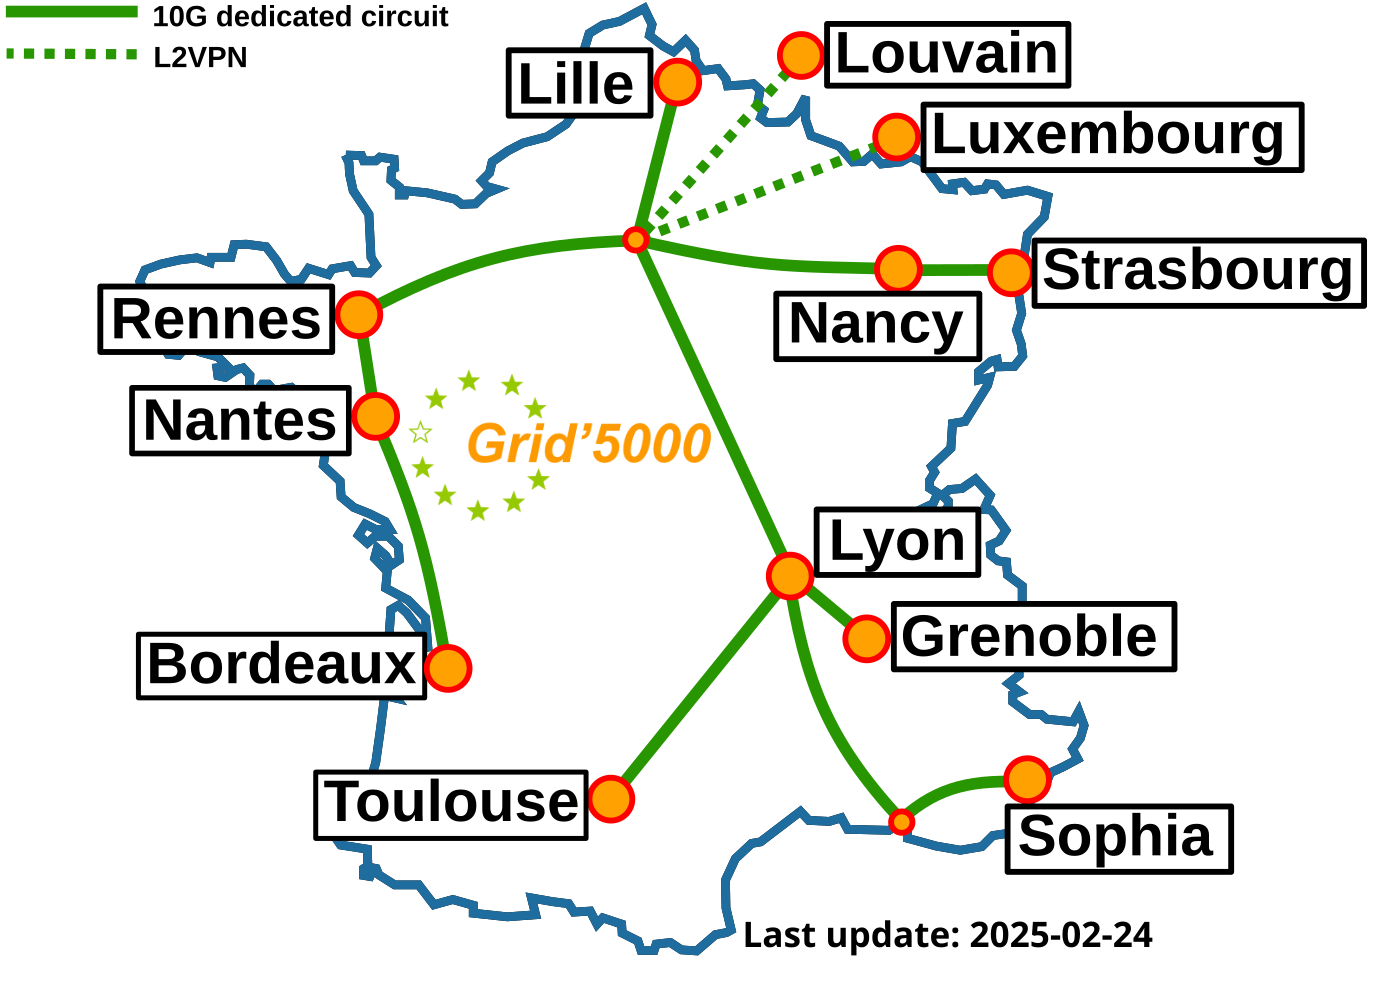
\includegraphics[height=2.5in]{images/G5k-backbone.png}
	\caption{Grid5000 testbed}
    \label{fig:grid5000}
\end{figure}

% Based on this taxonomy, one can more easily map an algorithm to an architecture in order to leverage the algorithm efficiency on this infrastructure. For instance, on heteregenous hardware systems (CPU + GPU

\textbf{Je penses qu'il serait bien d'avoir une conclusion et une transition ici}
%  les meilleurs environnements de programmation parallèle qui offrent le plus de puissance de calcul sont les
% environnements distribués, pouvoir les utiliser avec un modele de programmation approprié permet de resoudre
% des problèmes de très grande taille


\section{Programming environments (Programming model )}

% [ici il va falloir vraiment faire un peu le tour des différents environnements pour calcul distribué asynchrone]

% il n'y a pas de taxonomie reconnue qui permette de classer ces différents environnements 

% mais l'on peut faire une classification sur la base des standards de l'industrie qui refletent en meme temps les
% model de programmation en usage dans le domaine scientifique

In previous sections, we presented some taxonomy for parallel computing architectures. This preliminary work is of great importance, as the hardware infrastructure influences the choice of the programming environment when implementing parallel algorithms. Thus, many programming environments have emerged through years in order to map software to hardware infrastructure.

For parallel machines and local clusters, we can mention PVM, MPI and OpenMP. For distributed clusters, Global, Legion, Proactive, Padico. It is worth to mention that those list are not exhaustive and each environment is not exclusively related to one type of parallel architecture. 


For example MPI is worth using on supercomputers and local clusters, but  also efficient when it comes to distributed clusters, as the communication are done through message passing. In this section, we are presenting the MPI architecture and programming model, and discussing its gaps.

\hl{Maybe it can be instersting to talk about JACK here}


% nous allons nous focaliser sur ceux ayant ces caracterstiques
% etant un standard de l'industrie ou l'est devenu à l'usage
%  est portable sur plusieurs plateformes
% easy learning curve + high level code
% a de bonnes scalalability expectations
% represente un type de programming model
% possede une grande communauté - aide dans les projets
%  debugging and profiling tools maybe
% disponible dans plusieurs langages ( peut etre pas java)
% Must efficiently scale from multicore CPUs to thousands of nodes.
% deterministic




% 	•	Helps you choose the right tool based on algorithm structure and hardware.
% 	•	Allows you to compare environments like MPI, OpenMP, CUDA, Chapel in a structured way.
% 	•	Informs performance modeling and scalability expectations.




\subsection{OpenMP}
% Mentionner que openMP utilise plusieurs langages de programmation
% On peut egalement le combiner avec d'autres langages


OpenMP standing for Open Multi-Processing is an Application Programming Interface (API) that implement shared-memory programming paradigm for parallel programming on multi-core CPUs. The shared-memory programming paradigm that OpenMP implements implies that global memory is shared among threads while concurrent access are managed through synchronization mechanism in order to avoid data races, inconsistencies and undefined behavior. A common OpenMP program starts with a unique thread usually called the master thread. This unique thread is then fork (divided into multiple threads) whenever a parallel section is encounters in the algorithm implementation. Once the parallel section executed, the threads join back into the master. In order to keep consistency in global shared data among threads, some synchronization mechanism such as critical (protect a section from concurrent access), barrier(wait for all the threads to reach that point), reduction (combine result safely from multiple threads) to cite few, are available for the programmer. Other program control features of OpenMP include compiler directives, runtime routines and environment variables. Initiated in the late 1990's and maintened since then by the OpenMP Architecture Review Board (ARB), OpenMP has become a standard in industry thanks to it's easy to use, portability and scalability. The drawbacks of OpenMP lies in it's target. In fact OpenMP is only designed for shared-memory system, and does not provide parallelism for distributed system. Hence, the library does not scale across multiple nodes. Another industry-standard library provides this support with different programming paradigm.


\subsection{MPI - Message Passing Interface}

Message Passing Interface is a specification, based on the core concept of message passing, that gives guidelines for building an Application Programming Interface (API) intended to parallel programming. Historically, MPI arises in the early 1990s in order to define an industry standard that could solve the portability issues, due to vendor-specific message passing library.  Since then, the successive versions of the project, MPI-1 (1994), MPI-2 (1997), MPI-3 (2021) and MPI-4(2021) have defined many solutions along the initial portability solution, that made MPI the de facto standard for distributed memory systems. Non exhaustive list of MPI the key concepts are listed below.


\begin{description}

\item[Point-to-Point communication]  Communication operations that facilitate process interaction trough blocking (MPISend, MPIrecv … ) and non-blocking (MPIISend, MPIIRecv …)  operations.

\item[Collective communication] Operations that enable group communication (MPIBcast, MPIScatter, MPIGather …. )and often leveraging hardware accelerated interconnect features.

\item[Communicators and groups] These are abstractions that define groups (MPICOMMWORLD - abstraction for all the processes of an application ) of  processes and their communication context.

\item[Derived Datatypes] These enable efficient and portable communication of non-contiguous memory regions.

\end{description}

Consequently, MPI implementations (MPICH, openMPI…) became cornerstone for developing large, scalable and effecient applications… (continuer en demontrant quels aspects du developppement sont impactés, et conclure sur le futur de MPI, dire aussi comment certains aspects de mpi sont corrigés par des bibliothques exterieurs comme PETSc)



% \subsection{CUDA}



\subsection{Portable, Extensible Toolkit for Scientific Computation - PETSc}

\todo{mettre petsc apres la presentation des methodes numeriques}

% It supports an impressive range of systems including Windows NT/95.
% [ Presenter petsc, mais en rapport avec les besoins de la thèse ]

PETSc, the Portable, Extensible Toolkit for  Scientific Computation is a library designed to provide a highly abstracted framework for implementing large-scale (parallel) scientific applications modeled by partial differential equations (PDEs).  Initiated in the early 1990’s by the Argonne National Laboratory, the PETSc project was driven by the a key goal: provide an alternative to MPI and other programming model, that enables scientific to focus more on domain algorithm implementation than the low level task of parallelization. Consequently, the designed model filled the noticeable gaps of low level programming model such as the lack of data structure for distributed matrix and vectors, reusable solvers and preconditionners , and flexible run-time configurations options.

% [ Pourquoi avons nous choisit PETSc ? ]

PETSc library provides a good abstraction of some commonly used data structures in numerical solutions. Hence, IS, Vec, and Mat objects are respectively associated to index sets, vectors and matrices. An Index Set (IS) is a collection of integer indices that are used to identify subsets of parallel or sequential vectors and matrices, enabling user to work with local (per processor) and global (on all processors) indices on those data structures. Both matrix and vector object in PETSc are abstraction of common mathematical objects found in linear algebra, with sequential or parallel representation. Furthemore, those objects can be distributed across multiple processes, each one holding a local part of the data structure. Additionnaly to this data structure, the library provides many optimized routines that makes simple common linear algebra operations such as matrix-vector product ( MatMult ), matrix transposition (MatTranspose) and many more. When performing such operations that require multiple processes, PETSc automatically handles communication between those processes, based on the default  user-provided data layout. [transition sentence]


At a higher level in the abstraction layers of PETSc, we can find state-of-the-art solvers and preconditionners for numerical problems. In the context of systems of equations, a solver is an algorithm used to find an approximate or exact solution of the system, while a preconditionner is a transformation applied to system in order to improve the efficiency or the convergence of the solver. PETSc provides  linear (KSP), non-linear (SNES), time-dependent (TS) solvers, and indeed all those solvers can be use in a sequential or parallel manner, are re-usable, and can be combine to create more complex custom solvers. This framework of possibilities provide a ready to use environnement, that really ease the development of any simulation or algorithm.
Table 1 gives an overview of PETSc solvers and preconditionners.  [transition sentence]

% [Table 1]


Another great feature provided by PETSc, is the runtime configuration options. They are command line arguments or options database, that enable the user to control the behavior of PETSc applications at runtime, without modifying the source code. For example, the option database -kspsolver, provides a flexible and easy way to change the solver used to during the runtime, and could take any value corresponding to a petsc solver (gmres, cg …). Furthemore, one could easily change the memory layout of vector by changing its type, -vectype mpi corresponds to a distributed vector on CPU, while -vectype CUDA corresponds to a vector store on GPU. All this without changing any line of the source code. This feature really ease the development and experimental processes. 


%  [ Quels sont les potentiels challenges que ce choix implique ? ]

Though PETSc is a reliable alternative to low-level programming models, it’s come with some challenges. First, the API is large and complex, inducing a steep learning curve…….


\section{Performance metrics, evaluation}

%  [ Conclusion ]


\section{Conclusion}



% pages 5 - 14